\section{Trabalhos Relacionados}
\label{sec:trabalhosRelacionados}

De acordo com as fontes pesquisadas, especificapemente a bilioteca digital da IEEE, existem poucos trabalhos relacionados específicos à Smart IoT Gateway. 

O primeiro artigo \cite{designImplementationSIG} analisado possui similaridades com a nossa solução de Smart IoT Gateway, ele apresenta um software Smart Iot Gateway flexível que pode ser configurado para se adaptar a diferentes requisitos, e com isso reduzir custos e facilitar o ciclo de desenvolvimento. O Smart IoT Gateway tem como responsabilidade controlar os diferentes protocolos de comunicação, identificar os tipos de dispositivos e possíveis tratamentos de mensagens. Além disso, o gateway possui algumas interfaces externas unificadas, capazes de se adaptar à diferentes necessidades, onde os usuários podem desenvolver cartões apropriados de acordo com diferentes aplicativos. Como Ethernet (RJ45), USB, som e interfaces de vídeo, ver Figura~\ref{fig:arquiteturaDesignImpelementationSmartIoTGateway}.

\begin{figure}[h!]
	\begin{center}
		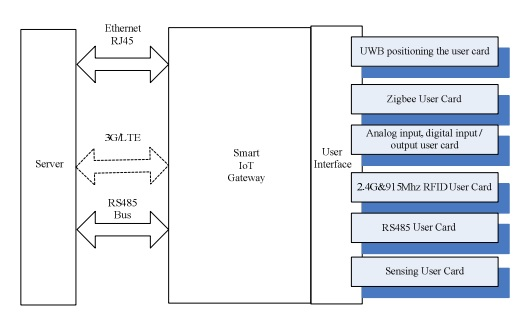
\includegraphics[width=0.8\textwidth]{./img/arquiteturaDesignImpelementationSmartIoTGateway}
		\caption{Arquitetura do Smart IoT Gateway. \cite{designImplementationSIG}}
		\label{fig:arquiteturaDesignImpelementationSmartIoTGateway}
	\end{center}
\end{figure}

Já o segundo artigo \cite{smartIotGatewayForHeterogeneous} também apresenta algumas similaridades com a nossa proposta. Propõe um Smart IoT Gateway que atua como um elemento central para conectar dispositivos através de protocolos e tecnologias de comunicação: ZigBee, Wifi, Bluetooth e Ethernet. Garante também a implementação das funcionalidades de conversão de protocolos, transformação, processamento e armazenamento de dados. Um dos aspectos que os autores destacam como trabalho futuro é a possibilidade de que usuários externos possam controlar remotamente os dispositivos heterogêneos como resposta a notificação de um evento.


